
\section{Experimentation}
\label{sec:experimentation}

\RPCBROADCAST proposes an original tradeoff in terms of complexity. Among other,
it removes the last monotonic and linear upper bound that remained on space
complexity. In this section, we evaluate the impact of the actual system on the
space consumed by processes. The experiments run on the \PEERSIM
simulator~\cite{montresor2009peersim} that allows to build large and dynamic
systems. Our implementation is available on the Github platform at
\url{http://github.com/chat-wane/peersim-prcbroadcast}. \\


% \begin{figure}
%   \begin{center}
%   
\begin{tikzpicture}[scale=0.6]

  \small
  
  \newcommand\X{1.45*\columnwidth/8pt};
  \newcommand\YA{0pt};
  \newcommand\YB{-60pt};


  \draw[->](0*\X, \YA) -- (9*\X, \YA);
  \draw[->](0*\X, \YB) -- (9*\X, \YB);
  
  \draw[fill=white] (0*\X, \YA) node{\textbf{\textup{A}}}
  +(-5pt, -5pt) rectangle +(5pt, 5pt);
  \draw[fill=white] (0*\X, \YB)  node{\textbf{\textup{B}}}
  +(-5pt, -5pt) rectangle +(5pt, 5pt);

  % \draw ( 1*\X, \YA ) node[above]{$\mathcal{A}$};
  % \draw ( 1*\X, \YB ) node[below]{$\mathcal{B}$};

  \draw[->] ( 2*\X, \YA ) -- node[sloped, above]{$\alpha$} (3*\X, \YB);
  % node[below left]{$\mathcal{A}$};

  \draw[decorate,decoration={brace,amplitude=6pt,mirror,raise=4pt}] (3*\X,
  -5+\YB) -- node[anchor=north, yshift=-10pt]{$B_{B\alpha}$}
  (5*\X, -5+\YB);

  % \draw ( 3*\X, \YA ) node[above]{$\mathcal{C}$};

  \draw[->] ( 3*\X, \YB ) -- node[sloped, above]{$\beta$} (4*\X, \YA);
  % node[above left]{$\mathcal{B}$};

  \draw[decorate,decoration={brace,amplitude=6pt,raise=4pt}] (4*\X,
  5+\YA) -- node[anchor=south, yshift=10pt]{$B_{A\beta} \bm{= B_{A\alpha}}$}
  (6*\X, 5+\YA);

  \draw[decorate,thick,decoration={brace,amplitude=6pt,raise=4pt}] (6*\X,
  5+\YA) -- node[anchor=south, yshift=10pt]{$\bm{B_{A\pi}}$}
  (8*\X, 5+\YA);
  
  
  % \draw ( 4*\X, \YB ) node[below]{$\mathcal{D}$};

  \draw[->] ( 4*\X, \YA ) -- node[sloped, above]{$\pi$} (5*\X, \YB);
  % node[below left]{$\mathcal{C}$};

  \draw[decorate,decoration={brace,amplitude=6pt,mirror,raise=4pt}] (5*\X,
  -5+\YB) -- node[anchor=north, yshift=-10pt]{$B_{B\pi} \bm{= B_{B\beta}}$}
  (7*\X, -5+\YB);


  % \draw ( 5*\X, \YA ) node[above]{$\mathcal{E}$};

  \draw[->] ( 5*\X, \YB ) -- node[sloped, above]{$\rho$} (6*\X, \YA);
  % node[above left]{$\mathcal{D}$};
  
  % \draw (6*\X, \YB) node[below]{$\mathcal{F}$};

  \draw[->, dashed] ( 6*\X, \YA ) -- node[sloped, above]{$B_{A\beta}$} (7*\X, \YB);

  \draw[->, dashed, thick] ( 7*\X, \YB ) --
  node[sloped, below]{$\bm{B_{B\beta}}$} (8*\X, \YA);

%  node[below left]{$\mathcal{E}$};


\end{tikzpicture}

%%% Local Variables:
%%% mode: latex
%%% TeX-master: "../paper"
%%% End:

%   \caption{\label{fig:bibroadcast}\RPCBROADCAST ensures the safety of bidirectional links
%     at marginal cost. Process~A maintains an additional buffer. Process~B transmits its
%     second buffer.}
%   \end{center}
% \end{figure}

% When links are bidirectional, \RPCBROADCAST must ensure their safety
% in both directions. Instead of performing twice \RPCBROADCAST's
% operation, we extend its behavior to handle bidirectional safety at
% once. Some control messages serve two purposes. For instance, control
% messages $\beta$ are also control messages $\alpha$. Some buffers have
% two purposes. For instance, the buffer $B_\beta$ of the process adding
% a link is also a buffer $B_\alpha$.  Figure~\ref{fig:bibroadcast}
% depicts the small change in the operation of \RPCBROADCAST. It ensures
% safety of bidirectional links at marginal cost compared to its
% unidirectional version. The buffer $B_\beta$ of Process~A becomes its
% buffer $B_\alpha$. The buffer $B_\pi$ of Process~B becomes a buffer
% $B_\beta$ that will be sent using the new link upon receipt of the
% buffer of Process~A. Between the sending of its buffer and the receipt
% of the buffer of Process~B, Process~A maintains an additional buffer
% $B_\pi$. \TODO{Maybe move this in proposal?}


\begin{figure}
  \begin{center}
    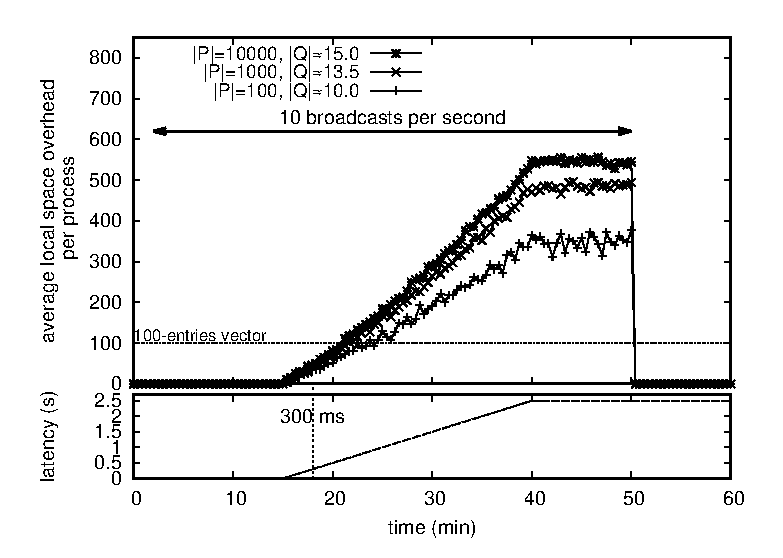
\includegraphics[width=0.8\columnwidth]{./img/overhead.eps}
    \caption{\label{fig:overhead}Local space overhead over time consumed by
      \RPCBROADCAST to ensure causal order and forbid double delivery in dynamic
      systems with varying latency.}
  \end{center}
\end{figure}


\noindent \textbf{Objective:} To confirm that local space complexity
depends on in-views and message receipts.

\noindent \textbf{Description:} We measure the average size of buffers and
arrays of expected messages. This constitutes the average local space overhead
consumed by \RPCBROADCAST to detect and forbid double delivery in dynamic
systems.\\
Runs involve 2 overlay networks comprising 100, 1k, and 10k
processes. \SPRAY~\cite{nedelec2017adaptive} builds an highly dynamic overlay
networks that allows balancing the traffic generated by broadcasting among
processes. Each process maintains a neighborhood logarithmically scaling with
the number of processes in the system. Each process of the 100-processes system
has a neighborhood of $\approx 10$ neighbors. Each process of the 1k-processes
system has a neighborhood of $\approx 13.5$ neighbors. Each process of the
10k-processes system has a neighborhood of $\approx 15$ neighbors. Each process
dynamically re-configure their neighborhood every minutes by exchanging safe
links with a chosen neighbor: it gives half of its safe links to the chosen
neighbor; the latter gives half of its safe links to the former as well. Each
exchange leads to safety checks of new links and removal of given links.\\ Links
are bidirectional, their safety must be checked in both directions but the
overhead remains minor. Links have transmission delay, i.e., the time between
the sending of a message and its receipt is not null. The experiments start with
$1ms$ delay. At $15min$ the delay starts to increase. At ~$17min$ links reach
$300ms$ delay. At $40min$
links reach $2.5s$ delay and it stops increasing.\\
From $2min$ to $50min$, every second, 10 processes chosen uniformly at random
among all processes broadcast a message.

\noindent \textbf{Results:} Figure~\ref{fig:overhead} shows the result of this
experiment. The x-axis denotes the time in minute. The top part of the figure
shows local space overhead while the bottom part of the figure shows the
evolution of transmission delays. 

\noindent Figure~\ref{fig:overhead} confirms that the local space consumption
  depends on the in-view size. Systems with larger in-views consume more
  space. Each new delivered message adds control information on each link of the
  in-view (see Algorithm~\ref{algo:reliablebroadcast}). 

\noindent Figure~\ref{fig:overhead} confirms that the local space consumption
  depends on network condition. The overhead increases as the latency
  increases. Latency increases the time between the first and the last receipt
  of each message. Processes store messages longer until they can be safely
  removed. 

\noindent Figure~\ref{fig:overhead} confirms that the local space consumption
  depends on broadcast messages. When processes stops broadcasting, the space
  consumed at each process drops to 0. Each process eventually receive each
  message and safely remove the corresponding entry.

\noindent Figure~\ref{fig:overhead} shows that at a rate of 10 broadcasts per second
  and when latency stays under a realistic bound ($300ms$), the overhead is
  lower than vector-based approaches. Whatever system conditions, it would
  require a vector of 100, 1k entries to forbid double delivery in the
  100-processes systems and 1k-processes system respectively. 

\noindent Overall, this experiment empirically confirms that the space
complexity of \RPCBROADCAST is non-monotonic and depends on the
system. Section~\ref{subsec:complexity} states that the space complexity is
$O(Q_i.M)$ where $Q_i$ is the size of the in-view built by peer-sampling
protocols, and $M$ is the number of messages that have been delivered but that
will be received again. This experiment shows that the space consumed by each
process increases and decreases over time.

\noindent In this experiment, the underlying peer-sampling protocol builds
random graph topologies that have numerous desirable properties such as crash
resilience, or load balancing~\cite{jelasity2007gossip}. This is ideal for
systems where numerous processes join and leave continuously. However, it is
worth noting that it remains in the hands of developers to choose the best
peer-sampling protocol for their system.

%Using \RPCBROADCAST, processes pay at the height of their current use instead of
%their past use.
The next section reviews state-of-the-art approaches designed to forbid multiple
delivery.




%%% Local Variables:
%%% mode: latex
%%% TeX-master: "../paper"
%%% End:
